%File: anonymous-submission-latex-2024.tex
\documentclass[letterpaper]{article} % DO NOT CHANGE THIS
\usepackage[submission]{aaai24}  % DO NOT CHANGE THIS
\usepackage{times}  % DO NOT CHANGE THIS
\usepackage{helvet}  % DO NOT CHANGE THIS
\usepackage{courier}  % DO NOT CHANGE THIS
\usepackage[hyphens]{url}  % DO NOT CHANGE THIS
\usepackage{graphicx} % DO NOT CHANGE THIS
\urlstyle{rm} % DO NOT CHANGE THIS
\def\UrlFont{\rm}  % DO NOT CHANGE THIS
\usepackage{natbib}  % DO NOT CHANGE THIS AND DO NOT ADD ANY OPTIONS TO IT
\usepackage{caption} % DO NOT CHANGE THIS AND DO NOT ADD ANY OPTIONS TO IT
\frenchspacing  % DO NOT CHANGE THIS
\setlength{\pdfpagewidth}{8.5in} % DO NOT CHANGE THIS
\setlength{\pdfpageheight}{11in} % DO NOT CHANGE THIS
%
% These are recommended to typeset algorithms but not required. See the subsubsection on algorithms. Remove them if you don't have algorithms in your paper.
\usepackage{algorithm}
\usepackage{algorithmic}

%
% These are are recommended to typeset listings but not required. See the subsubsection on listing. Remove this block if you don't have listings in your paper.
\usepackage{newfloat}
\usepackage{listings}
\DeclareCaptionStyle{ruled}{labelfont=normalfont,labelsep=colon,strut=off} % DO NOT CHANGE THIS
\lstset{%
	basicstyle={\footnotesize\ttfamily},% footnotesize acceptable for monospace
	numbers=left,numberstyle=\footnotesize,xleftmargin=2em,% show line numbers, remove this entire line if you don't want the numbers.
	aboveskip=0pt,belowskip=0pt,%
	showstringspaces=false,tabsize=2,breaklines=true}
\floatstyle{ruled}
\newfloat{listing}{tb}{lst}{}
\floatname{listing}{Listing}
%
% Keep the \pdfinfo as shown here. There's no need
% for you to add the /Title and /Author tags.
\pdfinfo{
/TemplateVersion (2024.1)
}

% DISALLOWED PACKAGES
% \usepackage{authblk} -- This package is specifically forbidden
% \usepackage{balance} -- This package is specifically forbidden
% \usepackage{color (if used in text)
% \usepackage{CJK} -- This package is specifically forbidden
% \usepackage{float} -- This package is specifically forbidden
% \usepackage{flushend} -- This package is specifically forbidden
% \usepackage{fontenc} -- This package is specifically forbidden
% \usepackage{fullpage} -- This package is specifically forbidden
% \usepackage{geometry} -- This package is specifically forbidden
% \usepackage{grffile} -- This package is specifically forbidden
% \usepackage{hyperref} -- This package is specifically forbidden
% \usepackage{navigator} -- This package is specifically forbidden
% (or any other package that embeds links such as navigator or hyperref)
% \indentfirst} -- This package is specifically forbidden
% \layout} -- This package is specifically forbidden
% \multicol} -- This package is specifically forbidden
% \nameref} -- This package is specifically forbidden
% \usepackage{savetrees} -- This package is specifically forbidden
% \usepackage{setspace} -- This package is specifically forbidden
% \usepackage{stfloats} -- This package is specifically forbidden
% \usepackage{tabu} -- This package is specifically forbidden
% \usepackage{titlesec} -- This package is specifically forbidden
% \usepackage{tocbibind} -- This package is specifically forbidden
% \usepackage{ulem} -- This package is specifically forbidden
% \usepackage{wrapfig} -- This package is specifically forbidden
% DISALLOWED COMMANDS
% \nocopyright -- Your paper will not be published if you use this command
% \addtolength -- This command may not be used
% \balance -- This command may not be used
% \baselinestretch -- Your paper will not be published if you use this command
% \clearpage -- No page breaks of any kind may be used for the final version of your paper
% \columnsep -- This command may not be used
% \newpage -- No page breaks of any kind may be used for the final version of your paper
% \pagebreak -- No page breaks of any kind may be used for the final version of your paperr
% \pagestyle -- This command may not be used
% \tiny -- This is not an acceptable font size.
% \vspace{- -- No negative value may be used in proximity of a caption, figure, table, section, subsection, subsubsection, or reference
% \vskip{- -- No negative value may be used to alter spacing above or below a caption, figure, table, section, subsection, subsubsection, or reference

\setcounter{secnumdepth}{0} %May be changed to 1 or 2 if section numbers are desired.

\usepackage{amsmath}
\usepackage{amssymb}
\usepackage{amsthm}
\usepackage{todonotes}
\usepackage{bm}
\usepackage{subcaption}
% \usepackage[ruled]{algorithm2e}

\def\ci{\perp\!\!\!\!\!\perp}

\newtheorem{definition}{Definition}
\newtheorem{proposition}{Proposition}
\newtheorem{theorem}{Theorem}


% The file aaai24.sty is the style file for AAAI Press
% proceedings, working notes, and technical reports.
%

% Title

% Your title must be in mixed case, not sentence case.
% That means all verbs (including short verbs like be, is, using,and go),
% nouns, adverbs, adjectives should be capitalized, including both words in hyphenated terms, while
% articles, conjunctions, and prepositions are lower case unless they
% directly follow a colon or long dash
\title{Title}
\author{
    %Authors
    % All authors must be in the same font size and format.
    Written by AAAI Press Staff\textsuperscript{\rm 1}\thanks{With help from the AAAI Publications Committee.}\\
    AAAI Style Contributions by Pater Patel Schneider,
    Sunil Issar,\\
    J. Scott Penberthy,
    George Ferguson,
    Hans Guesgen,
    Francisco Cruz\equalcontrib,
    Marc Pujol-Gonzalez\equalcontrib
}
\affiliations{
    %Afiliations
    \textsuperscript{\rm 1}Association for the Advancement of Artificial Intelligence\\
    % If you have multiple authors and multiple affiliations
    % use superscripts in text and roman font to identify them.
    % For example,

    % Sunil Issar\textsuperscript{\rm 2},
    % J. Scott Penberthy\textsuperscript{\rm 3},
    % George Ferguson\textsuperscript{\rm 4},
    % Hans Guesgen\textsuperscript{\rm 5}
    % Note that the comma should be placed after the superscript

    1900 Embarcadero Road, Suite 101\\
    Palo Alto, California 94303-3310 USA\\
    % email address must be in roman text type, not monospace or sans serif
    proceedings-questions@aaai.org
%
% See more examples next
}

%Example, Single Author, ->> remove \iffalse,\fi and place them surrounding AAAI title to use it
\iffalse
\title{My Publication Title --- Single Author}
\author {
    Author Name
}
\affiliations{
    Affiliation\\
    Affiliation Line 2\\
    name@example.com
}
\fi

\iffalse
%Example, Multiple Authors, ->> remove \iffalse,\fi and place them surrounding AAAI title to use it
\title{My Publication Title --- Multiple Authors}
\author {
    % Authors
    First Author Name\textsuperscript{\rm 1},
    Second Author Name\textsuperscript{\rm 2},
    Third Author Name\textsuperscript{\rm 1}
}
\affiliations {
    % Affiliations
    \textsuperscript{\rm 1}Affiliation 1\\
    \textsuperscript{\rm 2}Affiliation 2\\
    firstAuthor@affiliation1.com, secondAuthor@affilation2.com, thirdAuthor@affiliation1.com
}
\fi


\begin{document}

\maketitle

\begin{abstract}
	% TODO: Needs to be shortened.
	% In Pearl's framework, the initial step for performing a causal analysis
	% involves determining the causal structure between the variables from
	% data typically in the form of a Directed Acyclic Graph (DAG) or an
	% Structural Equation Model (SEM). This procedure, known as \emph{causal
	% discovery}, has been extensively studied for both DAGs and SEMs. While
	% numerous automated algorithms exist for estimating DAGs from datasets,
	% their application in applied fields remain limited, possibly due to a
	% lack of confidence in these algorithms stemming from them making
	% obvious mistakes, and the difficulties in choosing the right algorithm
	% for a given dataset. Consequently, in applied disciplines, these DAGs
	% are predominantly constructed manually based on domain expertise. Due
	% to being constructed by hand, it is vital that the fit of these models
	% are tested against data and the models are potentially modified to
	% acheive a better fit. On the other hand, in the field of SEMs models
	% are typically constructed manually through an iterative process of
	% assessing fit and modifying the model according to that. This process
	% is commonly known as \emph{Specification Search} where methods like
	% \emph{modification indices} combined with expert knowledge can be used
	% to guide this modification process. In the case of DAGs, although there
	% are tests to assess the global fit of a model by combining the tests
	% using implied conditional independencies of the model, but there are no
	% methods that can guide our modification process. In this paper, we
	% present a simple modification process aimed at helping researchers in
	% manually constructing or modifying DAGs outputted by an algorithm. This
	% modification process is based on using a (conditional) measure of
	% association between variables in the model to assess potential edges
	% that best explains unexplained correlation between variables which the
	% researcher specifies the direction of this edge. In the case of
	% continuous or discrete variables, the effect size measures of local
	% tests can be used as this measure of association, however for mixed
	% data there is no such measure. We present a measure of association
	% based on canonical correlations for mixed data. We also present a
	% graphical web-tool that can assist researchers in iteratively modifying
	% and constructing their DAGs. We theoretically show that in the presence
	% of an oracle, this iterative modification process is consistent in
	% recovering the true DAG. Emprically, we show that using the mixed data
	% measure of association, the modification process performs comparably to
	% PC and Hill-Climb Search algorithms if the user is able to correctly
	% identify the direction of the edge in one out of three cases.
\end{abstract}

\section{Introduction}

Understanding cause-and-effect relationships between variables is a fundamental
goal in many scientific questions as it reveals the underlying mechanisms of
the observed phenomena and informs effective interventions or policy decisions.
\emph{Causal Discovery} methods aim to uncover the underlying causal structure
among random variables from a given observational dataset. The problem of
causal discovery has been explored in both the Directed Acyclic Graphs (DAGs)
and Structural Equation Models (SEMs) literatures, each with different
approaches. In the DAG literature, the focus has been on developing automated
algorithms that can learn the causal structure from observational datasets. In
contrast, the SEM literature focuses on tools that help researchers manually
construct or modify models.

% To perform any causal effect identification or estimation using Directed
% Acyclic Graphs (DAGs) or Structural Equation Models (SEMs), researchers need to
% first construct a causal structure commonly known as DAG or path diagram. This
% process of constructing the casual structure from data is known as \emph{Causal
% Discovery}. In the field of DAGs, plenty of algorithms have been developed to
% automatically construct DAGs from data. These algorithm takes different
% approaches to causal discovery such as Constraint-based algorithms such as PC
% and Fast Causal Infenrece (FCI) where the algorithm tries to match the
% conditional independences in the data to the ones impled by the model,
% score-based methods such as Hill-Climb Search, Greedy Equivalence Search (GES)
% where the algorithm tries to find a model that has the best score given some
% scoring metric, and continuous optimization where the problem is formulated as
% a constrained optimization problem such as No Tears.

In the DAG literature, many automated algorithms have been developed for causal
discovery such as constraint based methods like PC \citep{Spirtes2001} and FCI
\citep{Spirtes2000}, score-based methods like Hill-Climb Search, Greedy
Equivalence Search \citep{Chickering2002}, and optimization based methods.
However, the adaption of these algorithms in applied fields remain limited
\citep{Tennant2020}. Researchers in applied fields typically prefer to
construct DAGs manually based on their domain knowledge. We hypothesize that
this preference towards manual DAG construction stems from the following
challenges in applying causal discovery algorithms: 

\begin{enumerate}
	\item \textbf{Trustworthiness: } Although most algorithms have
		asymptotic theory proving them to be consistent, their finite
		sample properties are not well understood. Moreover, depending
		on the selected hyperparameters of the algorithms, the output
		can vary very significantly. In real-world settings with finite
		samples, these algorithms can make obvious mistakes, for
		example, the constraint-based algorithms are biased towards
		sparse graphs \citep{Malinsky2024}. Consequently, researchers
		often have rely on post-hoc modifications based on model
		testing methods and their domain knowledge.
	\item \textbf{Outputs Markov Equivalence Class (MEC):} Multiple causal
		structures can be faithful to a given observational dataset.
		Thus, using only observational data, these algorithms can only
		recover the MECs that can contain unoriented edges. However,
		most methods for downstream tasks, such as identification or
		causal effect estimation, assume knowledge of a fully oriented
		DAG. As a result, researchers have to rely on their expertise
		to orient these edges or make further assumptions to make use
		of pairwise orientation techniques.
	% \item \textbf{Algorithm and hyperparameter selection:} Each algorithm
	% 	has the same goal but they can learn very different models
	% 	depending on the choice of algorithm and their hyperparameters.
	% 	For example, the choice of the conditional independence (CI)
	% 	test being used for constraint-based method depends on the
	% 	dataset, similarly for the scoring method for score-based
	% 	methods. With no obvious way to test the impact/performance of
	% 	these choices on a given dataset, it becomes quite hard to
	% 	chose the optimal algorithm for a given dataset.
\end{enumerate}

As a result of these challenges, doesn't matter if the researcher is manually
constructing the DAG or using an algorithm, they need to do some manual
modifications to the model before being able to use them for analysis. One of
the common ways to guide this modification is to use Conditional Independence
(CI) based model testing \cite{Ankan2021}. As DAGs imply CI statements that can
be tested in the given data, and then model can be modified based on the
p-values of these test. Figure~\ref{fig:ci_testing} shows an example of testing
using CIs. This approach has two main drawbacks:
\begin{enumerate}
	\item CIs are implied by missing edges only, and hence we can not test
		whether an incorrect edge is present in the model.
	\item For larger graphs, the number of CI tests can be very large, for
		example, the alarm network with $ 37 $ nodes has $ 287 $
		implied CIs. It can be difficult to look at all these tests for
		violations.
\end{enumerate}

% As it is evident that researchers also draw DAGs by hand and even if they use
% an algorithm, the need to make some post-hoc adjustments to the model, in this
% paper we present a tool to assist researchers in making these adjustments
% somewhat inspired by modification indices. In the case of DAGs, global testing
% methodology does exist such as Shipley test, that can combine local structure
% tests into a single p-value test. However, this does not give us a way to make
% modifications to our model. A possible way to do this by checking which of
% these local tests are violated. However, this approach can quickly become
% diffult as the size of the network increases. For example, the popular alarm
% network implies $x$ condition independence statements.

On the other hand, in Structural Equation Models (SEMs) literature, more
emphasis has been placed on helping researchers manually construct models while
integrating their expertise. Researchers typically develop an initial model
based on domain knowledge and use various tools to guide modifications to
improve the fit of their model to data while it still making theoretical sense.
This model construction process is known as \emph{Specification Search}. A
common method for specification search is \emph{modification indices}, which
identify potential changes to the model structure that improve the model fit
and ranks them using the most improvement to the model fit. This ranking allows
the researchers to focus first on the suggestions that can improve the model
the most and while integrating their expertise to choose the most optimal
modifications.

\todo[inline]{Show a figure of how the output looks like for modification indices}
\todo[inline]{Other methods: Modification indices and Lagrange Multiplier tests to
selectively add edges And using Wald test or z statistics (also known as
critical ratios) for removing edges.}

Inspired by this ranking approach, in this paper we present a way to rank the CI 
testing using a measure of association. This can be interpreted as the edge 

Our proposed approach uses a measure of association to find correlated variables
in the data that are not explained by the current model. Using the measure, we 
can rank the edge that can lead to the highest explanation of the observed 
correlation. Based on this information, the user can select a potential edge
and based on their expert knowledge decide the direction of the edge.

% We present a similar procedure for modifying DAGs based on expert knowledge and
% measure of association. We first use the measure of association to test whether
% the association observed in the data is explained by the model structure. We
% can not directly use the local CI tests to make modifications because that
% would give way too many independencies and we have no way to rank them. Based
% on this testing, we suggest adding edges by ranking them by the most
% unexplained association between variables. The researcher can then use expert
% knowledge to decide the direction of the edge between the variables.

Our main contributions in this papers are as follows:
\begin{enumerate}
	\item We present a measure of (conditional) association for mixed data
		based on canonical correlations. This measure of association
		generalizes the widely used partial correlation to mixed data
		setting.
	\item Using this association measure, we present a procedure to suggest
		modifications (i.e., new edges, and deleting edges) to a given
		model such that the model can better explain the observed
		associations in the data. 
	\item Lastly, we present a web-browser based tool to allow researchers
		to apply this method to their own datasets.
\end{enumerate}

\begin{figure}
	\centering
	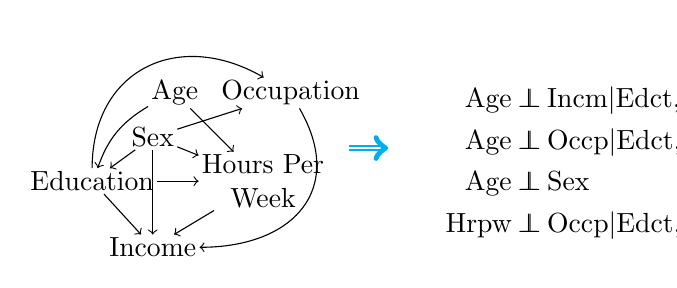
\begin{tikzpicture}
		\begin{scope}[xshift=-2.5cm, yshift=0.7cm, scale=0.7]
			\tikzstyle{every node}=[align=center, inner sep=1pt]
			\node (sex) at (-0.7, -0.8) {Sex};
			\node (age) at (-0.3, 0) {Age};
			\node (ed) at (-1.8, -1.6) {Education};
			\node (occ) at (1.8, 0) {Occupation};
			\node (hrpw) at (1.3, -1.6) {Hours Per \\ Week};
			\node (income) at (-0.7, -2.8) {Income};
		
			\draw[->]  (age) to[bend right=20] (ed);
			\draw[->]  (sex) to (ed);
			\draw[->]  (age) to (hrpw);
			\draw[->]  (ed) to (hrpw);
			\draw[->]  (sex) to (hrpw);
			\draw[->]  (ed) to (income);
			\draw[->]  (hrpw) to (income);
			\draw[->]  (occ) to[out=300, in=0, looseness=1.4] (income.east);
			\draw[->]  (sex) to (income);
			\draw[->]  (ed) to[out=90, in=150, looseness=1.3] (occ);
			\draw[->]  (sex) to (occ);	
		\end{scope}
		\begin{scope}[xshift=-3cm]
			\draw[thick, ->, double, cyan] (2.5,0) -- (3,0);
			\node[rectangle, align=center, inner sep=1pt] at (5, 0) {
				\begin{minipage}{.2\textwidth}
					\begin{equation*}
						\begin{split}
							\textnormal{Age} &\ci \textnormal{Incm} \rvert \textnormal{Edct, Hrpw, Sex} \\
							\textnormal{Age} &\ci \textnormal{Occp} \rvert \textnormal{Edct, Sex} \\
							\textnormal{Age} &\ci \textnormal{Sex} \\
							\textnormal{Hrpw} &\ci \textnormal{Occp} \rvert \textnormal{Edct, Sex} \\
						\end{split}
					\end{equation*}
				\end{minipage}
				};
		\end{scope}
		\end{tikzpicture}
		\caption{\todo[inline]{Finish figure to show an example of model testing}}
		\label{fig:ci_testing}
\end{figure}
\begin{figure}
	\caption{\todo[inline]{Placeholder for figure showing an example of modification indices}}
\end{figure}

The rest of the paper is structured as follows. In
Section~\ref{sec:background}, we give a background on the measures of
association for various data types. In Section~\ref{sec:mixed_association}, we
present our method for computing mixed data association. In
Section~\ref{sec:modification} and Section~\ref{sec:}, we present how to use
this method to make modifications and the web tool, and lastly in
Section~\ref{sec:empirical}, we show some empirical analysis on how well this
modification process works.

\section{Background and Related Work}
\label{sec:background}
We consider random variable $ X $ and $ Y $ with a possible multi-dimensional
variable $ \bm{Z} = \{ Z_1, \cdots, Z_k \} $. We consider these variables in
the mixed data setting where these variables can be any combination of
continuous, categorical, or ordinal unless specified. We use $ \rvert \bm{Z}
\rvert $ to represent the cardinality of the variable $ \bm{Z} $. We write $
\bm{x} = (x_1, \cdots, x_n) $ for a sample from $ X $ of size $ n $. We write
the expectation of a variable $ X $ as $ \mathbb{E}[X] $, conditional
expectations as $ \mathbb{E}[X | \bm{Z}] $.

We consider the problem of estimating the partial (or conditional) association
between $ X $ and $ Y $ in the presence of a set of conditioning variables $
\bm{Z} $. When $ Z = \emptyset $, this is equivalent to the marginal
association between $ X $ and $ Y $.

\todo[inline]{Add more notation as they come}

\subsection{Measures of (Conditional) Association}
As our DAG construction procedure relies on a measure of conditional
association between variables, in this section we list out some of the already
known measures for specific data types. These measure of associations are
typically the effect size of various conditional indepdnence tests but they
don't need to be. However, there are no generalized measure of association for
mixed data, that we propose in the next section. This is by no means an
exhaustive list, rather just to give an idea of what can be done.

\paragraph{Both $ X $ and $ Y $ are continuous}
Where there are no conditional variables, $ \bm{Z} = \emptyset $, Pearson's
correlation coefficient can be used as a measure of association between the
variables. This does make various assumptions such as linearity between the
variables, normal distribution for $ X $ and $ Y $, and homoscedasticity.

In the case when $ \bm{Z} \neq \emptyset $, then partial correlations can be
used. This requires using two linear regression models: $ E_X: X \sim \bm{Z} $
and $ E_Y: Y \sim \bm{Z} $. Then computing the residuals using these two
regressions as: $ R_X = X - E_X(\bm{Z}) $ and $ R_Y = Y - E_Y(\bm{Y}) $. After
this a simple correlation coefficient can be computed between $ R_X $ and $ R_Y $.

\paragraph{All $ X $, $ Y $, and $ \bm{Z} $ are discrete}

In the case of discrete variables, Cramer\'s V has been typically used as a
measure of association. When there are no conditional variables, $ \bm{Z} = \emptyset $,
Cramer\'s V can be computed directly from the contingency table.

However, when conditional variables are present, we can iterate over all
possible combinations of the conditional variables, compute the Cramer\'s V and
then lastly combine them together. 

\todo[inline]{Is it even possible}

\paragraph{$ X $ is ordinal and $ Y $ is continuous}
Polyserial Correlation

When $ \bm{Z} = \emptyset $, ordinal variable can be assumed to be coming from
a thresholded normal distribution, estimate the thresholds and latent variable
to compute the correlation coefficient.

\paragraph{$ X $ and $ Y $ are ordinal}
Polychoric Correlation

\section{A Measure of Association for Mixed Data}
\label{sec:mixed_association}

In this section, we define a novel partial measure of association for mixed
data by extending the idea of partial correlation to mixed data. We do this by
combining a mixed-data residualization method with a multivariate measure of
association. Given $ n $ samples $ D = (x, y, \bm{z}) $ of variables $ X $, $ Y $,
and $ \bm{Z} $, we are interested in computing an estimate of the conditional
association $ \rho(X, Y; \bm{Z}) $ between $ X $ and $ Y $ conditioned on $
\bm{Z} $. As the residualization approach requires atleast one conditional
variable to be present, if $ \bm{Z} = \emptyset $, we use a constant value for
$ Z $. Firstly, we compute the residuals for $ X $ and $ Y $ using the $ \bm{Z}
$ as the predictor variables. We use the mixed data residualization approach
from \citet{Ankan2023}. The residual computation depends on the type of 
variable:

\begin{enumerate}
	\item \textbf{$ X $ is continuous:} We start by training a regression
		model, $ E_X: x \sim \bm{z} $. Next we take the predictions
		from this model $ \hat{x} = E_X(\bm{z}) $ and lastly the
		residuals are computed as the difference between the true and
		the predicted values.
		$$ R_{x_i} = x_i - \hat{x}_i $$
	\item \textbf{$ X $ is ordinal:} We start by training a probability
		estimator, $ p_X: x \sim \bm{z} $, and take probability
		predictions from it $ \hat{p}_X: \hat{p}_X(\bm{Z}) $. Then we
		compute the residuals as follows:
		$$ R_{x_i} = \hat{p}(\hat{x}_i > x_i) - \hat{p}(\hat{x}_i < x_i) $$
	\item \textbf{$ X $ is categorical:} We again start by training a
		probability estimator $ p_X: X \sim \bm{Z} $, and take the
		probability estimates from it $ \hat{p}_X: p_Z(\bm{Z}) $. Next,
		we one-hot encode the categorical variable and then compute the
		residuals as follows: 
		$$ R_X = x_i - \hat{p}(\bm{z}_i) $$
\end{enumerate}

\todo[inline]{Fix notations above}

Here, users have the option to choose the estimators based on the properties of
their data. Non-parametric ensemble estimators such as Random Forest and
XGBoost can work well on a large variety of data and any data type. For linear
datasets users can also choose variants of linear regression depending on the
type of data. After the above steps are repeated for both $ X $ and $ Y $, we
end up with two residual matrices: $ R_X $ and $ R_Y $. The type of the
variable determines the shape for these matrices, i.e., if the variable is
continuous we get a residual matrix of shape $ ( n \times 1 ) $ and if the
variable is categorical we have a residual matrix of shape $ ( n \times (k-1))
$ (where one of the dummy encoded variables is dropped to avoid
multicollinearity)

We now have two continuous valued residual matrices and we need a measure to
quantify the association between these residuals. In multivariate statistics,
canonical correlation based measures have been used for measuring association
between two sets of variables. We can treat the residuals as sets of variables
in case of categorical variable and use canonical corrleations to quantify the
association between them.
\todo[inline]{Justify the argument}

\begin{definition}
	Given two sets of random variables $ \bm{U} = (U_1, U_2, \cdots, U_p) $
	and $ \bm{V} = (V_1, V_2, \cdots, V_q) $, canonical correlation between
	them, $\rho(\bm{U}, \bm{V}) $ is defined as:
		
	\begin{equation}
		\rho(\bm{U}, \bm{V}) = \sup_{a, b} \frac{a^T \Sigma_{\bm{U}\bm{V}} b}{\sqrt{a^T \Sigma_{\bm{U}\bm{U}} a} \sqrt{b^T \Sigma_{\bm{V}\bm{V}} b}}
	\end{equation}

\end{definition}
	
Canonical correlations are generalization of correlations to multi-dimensional
variables. It tries to find orthogonal linear transformations $ a $ and $ b $
of $ \bm{U} $ and $ \bm{V} $ such that the correlation between the transformed
variables $ a^T \bm{U} $ and $ b^T \bm{V} $ is maximized. It gives a vector of
correlation values of size $ \min(\rvert U \rvert, \rvert V \rvert) $
representing the correlation coefficient of each column of the transformed
variables. Pearson's correlation coefficient is a special case of canonical
correlations when $ \rvert U \rvert = \rvert V \rvert = 1$.

Many measures of association based on canonical correlation have been used in
multivariate statistics with each of them having slightly different properties.
\begin{itemize}
	\item Wilks' Lambda: $ \Lambda = \prod (1 - \phi_i^2) $
	\item Roy's Largest Root: $ \theta = \phi_{\max}^2 $
	\item Pillai's Trace: $ \tau = \sum \phi_i^2 $
\end{itemize}

We use Pillai's Trace for our purpose for two main reasons: 1) It uses all the
canoncial correlation values, 2) Its interpretation is similar to correlation
coefficient, i.e., $ 0 $ signifies no association and $ 1 $ signifies perfect
linear relationship. 

\todo[inline]{Add the formula for our case here}

This measure of association has many desired properties:

\begin{enumerate}
	\item Bounded between $ 0 $ and $ 1 $.
	\item Independent of sample size.
	\item Invariant to the one-hot encoding scheme used fr categorical variables.
	\item Reduces to partial correlations when both variables are continuous.
	\item In case of discrete variables, connected to Cramer\'s V, a well
		known effect size measure for discrete variables.
		\todo[inline]{Show the connection}
\end{enumerate}

\section{Using Measure of Association for DAG Modification and Construction}
\label{sec:modification}

% Add that we need a p-value as well.

Using this mixed data partial association measure, we propose an iterative DAG
modification procedure. 
\todo[inline]{How similar is this to GES algorithm}
If the user desires to construct the model manually, they can also start with
an empty graph. Given a DAG $ G $ and a dataset $ D $, for each pair for
variable $ X $ and $ Y $ in $ G $ that does not have an edge between them, we
compute the partial association measure: $ \rho(X, Y; pa_G(X) \cup pa_G(Y)) $.
The measure of association in this case can be interpreted as the unexplained
observed association between them given the current model. We can then use this
to rank pair of variables which have very high unexplained association between
them. Based on the domain expertise, the user can then choose one of these
suggested pair of variables, decide the direction of the edge between the
variables, and add it to the model. Once the new edge is added we can recompute
the association of all other variables and $ X $ and $ Y $.

Additionally, in each iteration of modification, for each pair of variable in $
G $, that has an edge between them in we compute the partial association
measure: $ \rho(X, Y; pa_{\underline{G}}(X) \cup pa_{\underline{G}}(Y) $. This
measure of association can be interpreted as the strength of the edge between
the variables. If the value of this association below a certain threshold, we
can remove the edge.

\begin{theorem}
	If we have access to an oracle that can give correct edge directions, taking a
	greedy approach with the procedure above results in the correct graph
	being recovered.
\end{theorem}

\section{Web Tool}
\label{sec:web}
Based on the procedure outlined in the previous section, we built a web-based
tool that allows users to interactively create/modify their model. The user
starts by uploading their dataset and optionally the initial DAG. If no initial
DAG is provided an empty graph is initialized. The tool also computes the
Shipley's C value at any point. The web-tool would automatically show all
unexplained associations in the DAG by adding red edges between them. The edge
weight of the edge represents how high this strength is. Users can also set the
threshold for p-value and association to control how many edges are shown at a
time. Based on these shown potential edges, the user can select the edge that
they want to add and decide the direction for it. If the tool detects an
incorrect edge in the graph, it is shown in black. Once the user is happy with
the graph they have they can export it into different formats to use it for
further computation.

% \begin{figure}
% 	\centering
% 	\begin{subfigure}{0.5\textwidth}
% 		\includegraphics[scale=0.25]{../../presentations/2024_05_das/2.png}
% 	\end{subfigure}%
% 	\begin{subfigure}{0.5\textwidth}
% 		\includegraphics[scale=0.25]{../../presentations/2024_05_das/5.png}
% 	\end{subfigure}
% 	\caption{Screenshots of the web-tool. \todo[inline]{Insert screenshots of the web-tool}}
% \end{figure}

\section{Empirical Analysis}
\label{sec:empirical}

We analyzed the performance of this manual approach by comparing it with two
automated algorithms: PC and Hill-Climb Search. For the comparison we use
simulated data from a known DAG and compare how well the algorithm is able to
recover the original model using two metrics: Structural Hamming Distance (SHD)
and Structural Intervention Distance (SID). To simulate the data, we start with
a randomly generated DAG and use linear models with random effects to generate
the data. We repeat the data generation $ 30 $ times for each density value for
the DAG. As both PC and Hill-Climb Search can only give us a CPDAG, we compare
the orientation of these CPDAG which result in the best and worst case scores
on SHD and SID. This procedure is outlined in Algorithm 1.

\todo[inline]{Add the algorithm}

To simulate an expert using this assisted model construction approach, we start
with an empty model and take a greedy approach to add edges to this model. At
any point, we select the pair of variables that has significant correlation and
the highest unexplained correlation, i.e., highest conditional association. We
then use an oracle to decide the direction of the edge between the variables.
Given an accuracy of the oracle, $ \alpha $, the oracle either gives the
correct direction, incorrect direction, or returns None representing that it
does not know the direction.

\begin{equation}
	\begin{split}
		x &= \textnormal{rand}([0, 1]) \\
		O(\alpha) &= \begin{cases} 
			M \rightarrow Y, & \textnormal{if  } x <= \alpha \\
			\textnormal{rand}(M \rightarrow Y, M \leftarrow Y, None) & \textnormal{otherwise} \\
				\end{cases} \\
	\end{split}
\end{equation}

If the oracle returns None for any pair of variables, an edge between this pair
is not suggested to the oracle in future iterations. We also make sure that
only edges which do not form a cyclic in the graph are used to select the next
potential edge. After adding each edge, we also check if the p-value of any
existing edge shows independence. If that happens we remove that edge and
blacklist that edge, i.e., that edge is not prompted again during the run of
the algorithm. We repeat this procedure till the model explains all
correlations between the variables. There is a possibility that this greedy
expert gets stuck at incorrect graph structures as it does not do any
backtracking to fix its earlier mistakes. This procedure is outlined in the
Algorithm.
\todo[inline]{Add the algorithm}

\subsection{Results}
\begin{figure}
	\begin{subfigure}{0.5\textwidth}
		\centering
		\includegraphics{../code/plots/shd_ribbon.pdf}
		\caption{}
	\end{subfigure}
	\begin{subfigure}{0.5\textwidth}
		\centering
		\includegraphics{../code/plots/sid_ribbon.pdf}
		\caption{}
	\end{subfigure}
	\caption{Comparison of PC and Hill-Climb Search algorithms against
		manually drawn DAGs using the assistance method. As PC and
		Hill-Climb Search return the Markov Equivalence Class (MEC), we
		use the best and worst scoring orientation of the MEC to get
		the range of values. The human drawn values are done for
		multiple accuracy values of the oracle.}
\end{figure}

\subsection{Using Large Language Models as Experts}
A lot of recent work has focused on finding pairwise causal direction among
variables using Large Language Models. In this analysis, instead of using the
oracle to decide the direction of edges, we used GPT4 to give us the direction
of the edges based on description of the variables. As GPT4 has already
memorized many of these models, we encoded the variable names using a random
string and provided the description of the variable to let it decide the
direction of the edge.

\section{Conclusions}

\bibliography{references}
\end{document}
